\section{Novel-View Synthesis}

\begin{frame}{Novel-View Synthesis}
    \centering
    \begin{overlayarea}{\textwidth}{4.3cm}
        \resizebox{\linewidth}{!}{%
        \begin{tikzpicture}[
            box/.style={rectangle, draw=blue!60!black, fill=blue!10, rounded corners, thick, minimum width=2.8cm, minimum height=1cm, align=center, font=\scriptsize\bfseries},
            phase/.style={rectangle, draw=blue!80!black, fill=blue!5, thick, rounded corners=2pt, minimum width=2.2cm, minimum height=0.9cm, align=center, font=\scriptsize\bfseries},
            arrow/.style={-Latex, thick, blue!70!black, rounded corners=4pt}
        ]
            % --- Nodes ---
            \node[box, fill=green!10, draw=green!50!black] (scene) at (0.7, 1.5) {Final \\ 3D Scene};
            \node[phase] (p2) at (3.8, 1.5) {FP Phase 2\\3D Matrix};
            
            \node[box] (cam) at (7.0, 1.5) {Camera Matrix \\ (Novel View)};
            \node[phase] (p3) at (10.4, 1.5) {FP Phase 3\\Projection};
            \node[phase] (p4) at (13.4, 1.5) {FP Phase 4\\Tile Mapping};
            
            \node[phase] (p5) at (13.4, -0.8) {FP Phase 5\\Radix Sort};
            \node[phase] (p6) at (10.4, -0.8) {FP Phase 6\\Rasterization};
            \node[box, fill=orange!10, draw=orange!80!black] (img) at (7.0, -0.8) {Rendered \\ Frame};
            
            % --- Arrows ---
            \draw[arrow] (scene.east) -- (p2.west);
            \draw[arrow] (p2.east) -- (cam.west);
            
            \draw[arrow] (cam.east) -- (p3.west);
            \draw[arrow] (p3.east) -- (p4.west);
            \draw[arrow] (p4.south) -- (p5.north);
            \draw[arrow] (p5.west) -- (p6.east);
            \draw[arrow] (p6.west) -- (img.east);
            
            \draw[arrow] (img.north) -- node[left, font=\scriptsize, text=blue!80!black] {Next Frame} (cam.south);
            
            % --- Grouping Brackets/Labels ---
            \draw[gray!80!black, thick, dashed] (5.2, 2.5) rectangle (14.8, -1.8);
            \node[font=\small\bfseries, text=gray!80!black, fill=white, inner sep=2pt] at (10, 2.5) {Real-Time Feed-Forward Loop};
            
        \end{tikzpicture}%
        }
    \end{overlayarea}

    \begin{itemize}
        \justifying
        \item Because the scene geometry is finalized, the backward pass, Adaptive Density Control, and other components are completely disabled.
        \item Freed from the this overhead and running at the raw speed of the tile-based rasterizer, 3DGS quickly reaches real-time rendering levels.
    \end{itemize}

    \pdfcomment[opacity=0]{
        - Assuming the loss function converged, we now have the final reconstructed 3D scene available for rendering novel views. \textCR
        - In 3DGS, this is quite simple as all the steps required for NVS are already there. (describe) \textCR
        \textCR
        - This concludes the presentation on 3D Gaussian Splatting. We've seen that ... \textCR
        (- videos?)
    }
\end{frame}

\section{Summary and Discussion}

\begin{frame}{Summary and Discussion}
    \begin{itemize}
        \justifying
        \item 3D Gaussian Splatting is a learnable and explicit radiance field representation for 3D Reconstruction, abandoning neural networks.\vspace{0.5em}
        \item Kerbl et al. combined multiple existing approaches and technologies, added new ideas, and mapped them onto modern GPU hardware.\vspace{0.5em}
        \item We analyzed the training procedure showing in detail how Kerbl. et al made it possible to have real-time rendering of reconstructed 3D scenes for the first time.
    \end{itemize}
    \vspace{3em}
    \centering
    Thank you for your attention. I am looking forward to taking your questions.
    \pdfcomment[opacity=0]{
        - Auch auf deutsch! \textCR
        - Hinweis auf Videos
    }
\end{frame}

\appendix

\section{Videos}

\begin{frame}{3DGS Videos}
    \begin{columns}[T]
        \begin{column}{0.5\textwidth}
            \centering
            \textbf{Training in Progress}
            \vspace*{1em}\\            
            \url{https://youtu.be/F9rgbvhSad8?t=550}\\
            \href{https://youtu.be/F9rgbvhSad8?t=550}{%
                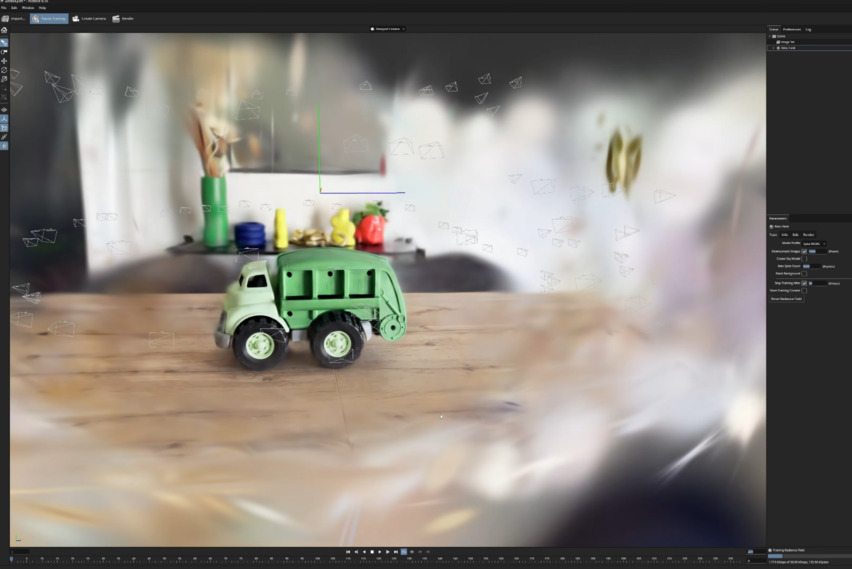
\includegraphics[width=0.65\linewidth]{figures/video_screenshot_truck.jpg}%
            }\\
            \vspace{1em}
            \url{https://youtu.be/yd40zUnr7eQ}\\
            \href{https://youtu.be/yd40zUnr7eQ}{%
                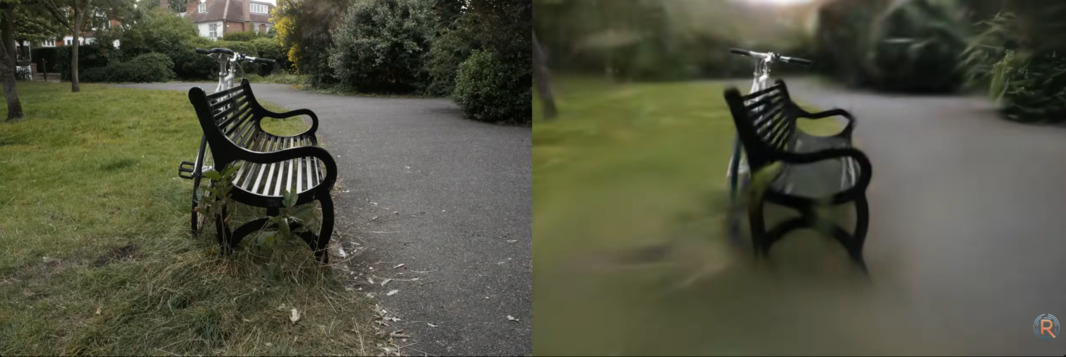
\includegraphics[width=0.65\linewidth]{figures/video_screenshot_bench.jpg}%
            }
        \end{column}
        \begin{column}{0.5\textwidth}
            \centering
            \textbf{Real-Time Rendering}
            \vspace*{1em}\\
            Example from the original paper's\\ project website
            \vspace*{1em}\\
            \url{https://repo-sam.inria.fr/fungraph/3d-gaussian-splatting/content/videos/bicycle.mp4}\\
            \href{https://repo-sam.inria.fr/fungraph/3d-gaussian-splatting/content/videos/bicycle.mp4}{%
                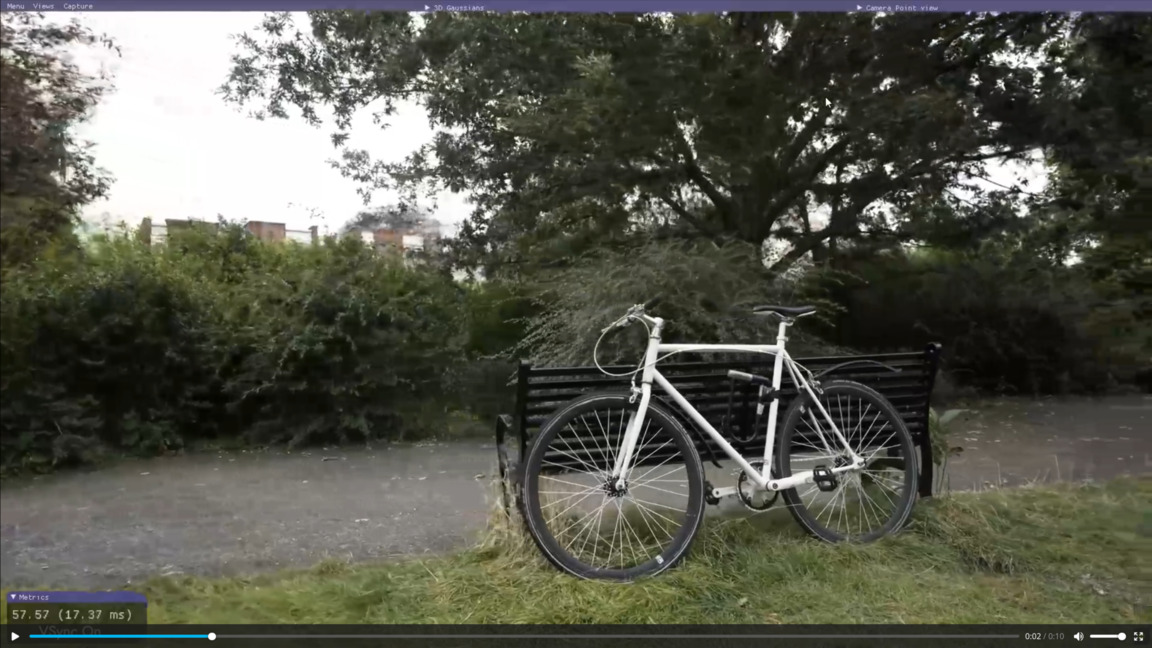
\includegraphics[width=0.7\linewidth]{figures/video_screenshot_bicycle.jpg}%
            }
        \end{column}
    \end{columns}
    \pdfcomment[opacity=0]{
        https://youtu.be/F9rgbvhSad8?t=550 \textCR
        https://youtu.be/yd40zUnr7eQ \textCR
        https://repo-sam.inria.fr/fungraph/3d-gaussian-splatting/content/videos/bicycle.mp4 \textCR
    }
\end{frame}

% \section{Backpropagation Gradient Flow}

% \begin{frame}[label=gradient_flow]{Backward Pass: Gradient Flow Overview}
%     \centering
    
%     % Wraps the TikZ diagram to ensure it fits the slide width perfectly
%     \resizebox{\linewidth}{!}{%
%     \begin{tikzpicture}[
%         % Styles for variables and arrows
%         var/.style={circle, draw=blue!60!black, fill=blue!10, thick, minimum size=1.1cm, inner sep=0pt, font=\small\bfseries},
%         varfirst/.style={circle, draw=blue!60!black, thick, minimum size=1.1cm, inner sep=0pt, font=\small\bfseries},
%         endvar/.style={circle, draw=green!60!black, fill=green!10, thick, minimum size=1.1cm, inner sep=0pt, font=\small\bfseries},
%         arrow/.style={-Latex, thick, blue!70!black},
%         header/.style={font=\footnotesize\bfseries, text=gray, align=center}
%     ]
%         % Column Headers
%         \node[header] at (0, 3) {Loss};
%         \node[header] at (2.2, 3) {Phase 1\\Color Error};
%         \node[header] at (4.6, 3) {Phase 2\\2D Splat};
%         \node[header] at (7.2, 3) {Phase 3\\2D Geometry};
%         \node[header] at (9.6, 3) {Phase 4\\Unprojection};
%         \node[header] at (12, 3) {Phase 5\\Attributes};
        
%         % Draw light vertical separators to distinguish phases
%         \foreach \x in {1.1, 3.4, 5.9, 8.4, 10.8} {
%             \draw[dashed, gray!30] (\x, 3.3) -- (\x, -3.8);
%         }

%         % --- Nodes ---
%         \node[varfirst] (L) at (0, 0.3) {$L$};
%         \node[var] (Cp) at (2.2, 0.3) {$C_p$};
        
%         \node[endvar] (ci) at (4.6, 1.8) {$c_i$};
%         \node[var] (alpha) at (4.6, -0.7) {$\alpha_i$};
        
%         \node[var] (mu2D) at (7.2, 0.8) {$\mu_{2D}$};
%         \node[var] (Sigma2D) at (7.2, -0.7) {$\Sigma_{2D}$};
%         \node[var] (o) at (7.2, -2.2) {$o$};
        
%         \node[endvar] (mu3D) at (9.6, 0.8) {$\mu_{3D}$};
%         \node[var] (Sigma3D) at (9.6, -0.7) {$\Sigma_{3D}$};
        
%         \node[endvar] (sraw) at (12, 0.1) {$s_{raw}$};
%         \node[endvar] (qraw) at (12, -1.5) {$q_{raw}$};
%         \node[endvar] (oraw) at (12, -2.9) {$o_{raw}$};
        
%         % --- Edges (Gradient Flow) ---
%         \draw[arrow] (L) -- (Cp);
%         \draw[arrow] (Cp) -- (ci);
%         \draw[arrow] (Cp) -- (alpha);
%         \draw[arrow] (alpha) -- (mu2D);
%         \draw[arrow] (alpha) -- (Sigma2D);
%         \draw[arrow] (alpha) -- (o);
%         \draw[arrow] (mu2D) -- (mu3D);
%         \draw[arrow] (Sigma2D) -- (Sigma3D);
%         \draw[arrow] (Sigma3D) -- (sraw);
%         \draw[arrow] (Sigma3D) -- (qraw);
%         \draw[arrow] (o) -- (oraw);
        
%         % --- Legend ---
%         \node[var, minimum size=0.5cm] at (1.5, -3.4) {};
%         \node[right, font=\scriptsize] at (1.8, -3.4) {Intermediate Gradient};
        
%         \node[endvar, minimum size=0.5cm] at (6.5, -3.4) {};
%         \node[right, font=\scriptsize] at (6.8, -3.4) {Final Attribute Gradient};
        
%     \end{tikzpicture}%
%     }
% \end{frame}

\section{Backpropagation Calculations}

\begin{frame}{Backward Pass Phase 3 (Part 1)}
    \textbf{Phase 3: 2D Splat to 2D Geometry (Opacity \& Position)}
    \begin{itemize}
        \item We recall the simplified opacity distribution: $\alpha_i(p) = o \cdot e^E$, where $E$ is the exponent derived from the pixel distance $\Delta$ and the inverse 2D covariance matrix.
        \item \textbf{Base Opacity ($o$):} The derivative scales directly with the distance from the center of the 2D Gaussian ($e^E$):
        $$ \frac{\partial L}{\partial o} = \frac{\partial L}{\partial \alpha_i} \cdot e^E $$
        \item \textbf{Position ($\mu_{2D}$):} Let vector $v = \Sigma_{2D}^{-1}\Delta p$. This vector points directly from the 2D Gaussian's center to the pixel:
        $$ \frac{\partial L}{\partial \mu_{2D}} = \frac{\partial L}{\partial \alpha_i} \cdot \alpha_i(p) \cdot v $$
        \item If the evaluated opacity gradient is positive, the center is effectively pulled towards the pixel.
    \end{itemize}
\end{frame}

\begin{frame}{Backward Pass Phase 3 (Part 2)}
    \textbf{Phase 3: 2D Splat to 2D Geometry (Shape)}
    \begin{itemize}
        \item \textbf{2D Covariance Matrix ($\Sigma_{2D}$):} We must calculate how the opacity at pixel $p$ changes when the 2D shape of the Gaussian changes.
        \item This uses the same vector $v$ from the position derivative, multiplied by its own transpose:
        $$ \frac{\partial L}{\partial \Sigma_{2D}} = \frac{\partial L}{\partial \alpha_i} \cdot \frac{1}{2} \alpha_i(p) \cdot (v \cdot v^T) $$
        \item Multiplying the vector by its transpose results in a matrix gradient.
        \item If the evaluated opacity gradient is positive, this matrix gradient causes the 2D Gaussian to stretch itself towards the pixel; otherwise, it causes it to contract.
    \end{itemize}
\end{frame}

\begin{frame}{Backward Pass Phase 4}
    \textbf{Phase 4: 2D Geometry to 3D Geometry}
    \begin{itemize}
        \item The GPU thread model changes to running per-Gaussian to unproject the 2D data back into 3D.
        \item This utilizes the multi-variable chain rule and the transposes of the forward projection matrices ($U = JW_{rot}$).
        \item \textbf{3D Position ($\mu_{3D}$):} The gradient passes through view space ($t$) back to world space:
        $$ \frac{\partial L}{\partial \mu_{3D}} = W_{rot}^T J^T \frac{\partial L}{\partial \mu_{2D}} = U^T \left( \frac{\partial L}{\partial \mu_{2D}} \right) $$
        \item \textbf{3D Covariance ($\Sigma_{3D}$):} The final gradient unprojects cleanly using matrix $U$ on both sides:
        $$ \frac{\partial L}{\partial \Sigma_{3D}} = U^T \left( \frac{\partial L}{\partial \Sigma_{2D}} \right) U $$
    \end{itemize}
\end{frame}

\begin{frame}{Backward Pass Phase 5 (Part 1)}
    \textbf{Phase 5: 3D Geometry to Matrix Components}
    \begin{itemize}
        \item Gradients flow through the covariance matrix assembly ($\Sigma_{3D} = MM^T$ with $M = RS$) into scale ($S$) and rotation ($R$).
        \item First, the algorithm derives the intermediate matrix $M$:
        $$ \frac{\partial L}{\partial M} = 2 \left( \frac{\partial L}{\partial \Sigma_{3D}} \right) M $$
        \item Then, it splits this gradient into the separate components:
        $$ \frac{\partial L}{\partial S} = R^T \left( \frac{\partial L}{\partial M} \right) \quad \text{and} \quad \frac{\partial L}{\partial R} = \left( \frac{\partial L}{\partial M} \right) S $$
        \item The scale gradient ($\frac{\partial L}{\partial s}$) is extracted from the diagonal of $\frac{\partial L}{\partial S}$, while the quaternion gradient ($\frac{\partial L}{\partial q}$) aggregates the partial derivatives of $R$.
    \end{itemize}
\end{frame}

\begin{frame}{Backward Pass Phase 5 (Part 2)}
    \textbf{Phase 5: Backpropagating to Latent Attributes}
    \begin{itemize}
        \item To close the loop, the gradients pass backwards through their respective activation functions to reach the raw, latent space variables.
        \item \textbf{Scale (Exponential):} Backpropagating through $\exp$ requires multiplying by $s$:
        $$ \frac{\partial L}{\partial s_{raw}} = \frac{\partial L}{\partial s} \cdot s $$
        \item \textbf{Rotation (Normalization):} Uses the Jacobian matrix ($J_{||}$) of the normalization function, with $J_{||} = \frac{I - qq^T}{||q_{raw}||}$:
        $$ \frac{\partial L}{\partial q_{raw}} = J_{||} \cdot \frac{\partial L}{\partial q} $$
        \item \textbf{Base Opacity (Sigmoid):} Backpropagating through the sigmoid function:
        $$ \frac{\partial L}{\partial o_{raw}} = \frac{\partial L}{\partial o} \cdot o(1-o) $$
    \end{itemize}
\end{frame}

\section{Selected References}

\begin{frame}[allowframebreaks]{Selected References}
    \footnotesize
    \nocite{*}
    \setbeamertemplate{bibliography item}[text]
    
    \bibliographystyle{plain}
    \bibliography{references}
\end{frame}